\section{Version Polymorphism}

% Copied this part from thesis' draft

\subsection{An Illustrating Example}

Let's illustrate this with a simple example involving different hashing algorithms defined in different versions. 
Listing~\ref{hash-class}\footnote{The code in this chapter does not include modifiers such as \texttt{public} for brevity.} 
shows version 1 and 2 of the class \texttt{Hash} that respectively implements MD5 and SHA-3 hashing algorithms written in \lang{}. 
The method \texttt{mkHash} hashes a \texttt{String} into a \texttt{HashValue}. Both versions are statically compatible with 
each other, meaning that each definition can replace the other version without breaking compilation. However, they are semantically 
incompatible because of the different algorithms. If a user intends to use any version of \texttt{Hash} in their program, 
they must not check a hash value generated in one version against a hash value generated from another version. 
To ensure that only the correct version of hash value is returned by and passed into \texttt{Hash}, 
the versions for each respective \texttt{HashValue} are fixed through \texttt{HashValue\#1\#} and \texttt{HashValue\#2\#}.

Suppose then that the hashing algorithm defined in \texttt{Hash} is used through a \texttt{Dir} class shown in Listing~\ref{dir-class} 
that can access files and check their contents. The method \texttt{exists} in \texttt{Dir} accepts a hash value \texttt{c}, hashes 
it with a specific hashing algorithm, and checks its equality with already stored files using \texttt{match}.

Under the assumption of programming with versions, users may want to use different versions of statically compatible \texttt{Hash} 
and \texttt{HashValue} through a single definition of \texttt{Dir}. In Listing~\ref{app-class}, an \texttt{App} class processing 
different types of string data through \texttt{Dir} may wish to use different versions of the algorithm as required. Due to possible 
constraints in the data storage, the user may need to use different algorithms in \texttt{processID} and \texttt{processLog}. Here, 
the IDs are processed using the older algorithm by passing a hash value generated from \texttt{new Hash\#1\#()}, while the logs are 
processed by the new algorithm with a hash value generated from \texttt{new Hash\#2\#()}.

However, compiling the program in \lang{} would result in:
\begin{lstlisting}[
    numbers=none,
    backgroundcolor=\color{backcolour}]
No solution found for the program
\end{lstlisting}


\begin{figure}[t]
\begin{lstlisting}[
    language=Java,
    caption=Two versions of \texttt{Hash} in \lang{},
    label=hash-class]
class Hash ver 1 {
  Hash() { }
  HashValue#1# mkHash(String s) {
    return new HashValue#1#(/* MD5 algorithm */);
  }
  boolean match(String s, HashValue#1# h) {
    return this.mkHash(s).equals(h);
  }
}

class Hash ver 2 {
  Hash() { }
  HashValue#2# mkHash(String s) {
    return new HashValue#2#(/* SHA-3 algorithm */);
  }
  boolean match(String s, HashValue#2# h) {
    return this.mkHash(s).equals(h);
  }
}
\end{lstlisting}

\begin{lstlisting}[
    language=Java,
    caption=\texttt{Dir} class using \texttt{Hash} and \texttt{HashValue},
    label=dir-class]
class Dir ver 1 {
  Dir() { }
  String[] getFiles() { /* retrieve stored strings */}
  boolean exists(HashValue c) {
    Hash hash = new Hash();
    for (String s: getFiles()) {
        if (hash.match(s, c) { return true; }
    }
    return false;
  }
}
\end{lstlisting}
\end{figure}

\begin{figure}[h!]
\begin{lstlisting}[
    language=Java,
    caption=\texttt{App} instantiating \texttt{Dir} with different versions,
    label=app-class]
class App ver 1 {
  boolean processID(String n) {
    // using MD5 algorithm
    return new Dir().exists(new Hash#1#().mkHash(n));
  }

  boolean processLog(String n) {
    // using SHA-3 algorithm
    return new Dir().exists(new Hash#2#().mkHash(n));
  }
}
\end{lstlisting}
\end{figure}

\section{Design}

The problem with \lang{} lies in its limited design that fixes the version for every class instance. To allow this reuse of 
the same definition, in other words, \emph{version polymorphism}, we have to relax this limitation in the original design of \lang{}.

A straightforward solution is to take a similar approach to Java generics~\cite{igarashi_featherweight_2001, bracha1998making}. 
In Java generics, types of fields or method arguments are polymorphised through type parameterizations to be made concrete 
during class instantiations or method invocations. The correctness of the 
type parameters and arguments are checked using their upper bounds as their type identities.

We follow the approach by extending \lang{} with version polymorphism through version parameterization. Version parameters abstract 
version assignments to class instances in the class definition and method declarations.

We illustrate this with the new class Dir in Listing~\ref{dir-class-poly} with polymorphic definition. The parameters \texttt{V} 
and \texttt{W} surrounded by the double angle brackets \texttt{<<>>} are version parameters declared for the class.
The version parameters are used by passing them to class access as version specifications inside the class definition. 
Class access refers to class annotations appearing in parameters and variable declarations such as \texttt{Hash\#V\# hash}. 
The class instance with sharp notation \texttt{Hash\#V\#} is similar in meaning to \texttt{Hash\#1\#} where the class instance 
Hash is specified to version \texttt{V}. Each version parameter is associated with a specific class. 
In \texttt{Dir}, \texttt{V} and \texttt{W} are respectively associated with the class \texttt{Hash} and \texttt{HashValue}.

Version polymorphic classes can be instantiated by passing version arguments during object instantiations. 
Listing~\ref{app-class-poly} shows the modified \texttt{App} using the polymorphic \texttt{Dir}. 
The two object instantiations for \texttt{Dir} in both \texttt{processID} and \texttt{processLog} are distinguished 
by the version arguments given to each instance through the angle brackets notation. In \texttt{processID}, the \texttt{Dir} 
object is instantiated by passing \texttt{<<1,1>>} as version arguments to \texttt{Dir}. This denotes that both \texttt{Hash} 
and \texttt{HashValue} in this object are set to version 1 and 1. Similarly, \texttt{<<2,2>>} is passed to \texttt{Dir} 
instantiation in \texttt{processLogs} denoting that \texttt{Hash} and \texttt{HashValue} are set to version 2 and 2. 

Unlike type parameters in Java generics, version parameters do not depend on version bounds for version checking. 
The compilation solves the set of solutions for the version parameters \texttt{V}, \texttt{W} and check 
the version arguments against these solutions. For the given example, the set of compatible solutions are
\begin{align*}
(\texttt{V}, \texttt{W}) \in \{ (1,1), (2,2) \}
\end{align*}
Hence, based on the solutions found, the two object instantiations for \texttt{Dir} in both \texttt{processID} and
\texttt{processLog} are well-typed. Conversely, incorrect object instantiations such as \texttt{new Dir<<1,2>>()} 
would be rejected.

A method declaration can also declare its own version parameters. The illustrating example can be rewritten 
by polymorphising the method declaration for \texttt{exists}. Listing~\ref{dir-method-poly} introduces 
version parameters \texttt{V} and \texttt{W} in method \texttt{exists}. Similarly as before, the parameters 
\texttt{V} and \texttt{W} are respectively associated with \texttt{Hash} and \texttt{HashValue}. 
Listing~\ref{app-method-poly} shows the version arguments being passed into \texttt{exists} invocations.

Note that in the current design we do not consider version polymorphic inheritance. 
This is because allowing polymorphic superclass definitions highly complicates a class structure. 
Although it is feasible to implement such a language, we consider 
leaving the burden of tracking which object inherits 
from which version of a class to the programmers to be disadvantageous.

\begin{figure}[h!]
\begin{lstlisting}[
    language=Java,
    caption=Polymorphic \texttt{Dir} class declaration,
    label=dir-class-poly]
class Dir ver 1 |\texttt{<<}|V,W|\texttt{>>}| {
  String[] getFiles() { /* retrieve stored strings */ }
  boolean exists(HashValue#W# c) {
    Hash#V# hash = new Hash#V#();
    for (String s: getFiles()) {
      if (hash.match(s, c)) { return true; }
    }
    return false;
  }
}
\end{lstlisting}

\begin{lstlisting}[
    language=Java,
    caption=\texttt{App} with polymorphic instantiations of \texttt{Dir},
    label=app-class-poly]
class App ver 1 {
  boolean processID(String n) {
    return new Dir|\texttt{<<}|1,1|\texttt{>>}|().exists(new Hash().mkHash(n));
  }
  boolean processLog(String n) {
    return new Dir|\texttt{<<}|2,2|\texttt{>>}|().exists(new Hash().mkHash(n));
  }
}
\end{lstlisting}
\end{figure}

\begin{figure}[h!]
\begin{lstlisting}[
    language=Java,
    caption=Polymorphic \texttt{exists} method declaration,
    label=dir-method-poly]
class Dir ver 1 {
  String[] getFiles() { /* retrieve stored strings */ }
  |\texttt{<<}|V,W|\texttt{>>}| boolean exists(HashValue#W# c) {
    Hash#V# hash = new Hash#V#();
    for (String s: getFiles()) {
      if (hash.match(s, c)) { return true; }
    }
    return false;
  }
}
\end{lstlisting}

\begin{lstlisting}[
    language=Java,
    caption=\texttt{App} with polymorphic invocations of \texttt{exists},
    label=app-method-poly]
class App ver 1 {
  boolean processID(String n) {
    return new Dir().|\texttt{<<}|1,1|\texttt{>>}|exists(new Hash().mkHash(n));
  }
  boolean processLog(String n) {
    return new Dir().|\texttt{<<}|2,2|\texttt{>>}|exists(new Hash().mkHash(n));
  }
}
\end{lstlisting}
\end{figure}

\section{Implementation}

\begin{figure}[h]
%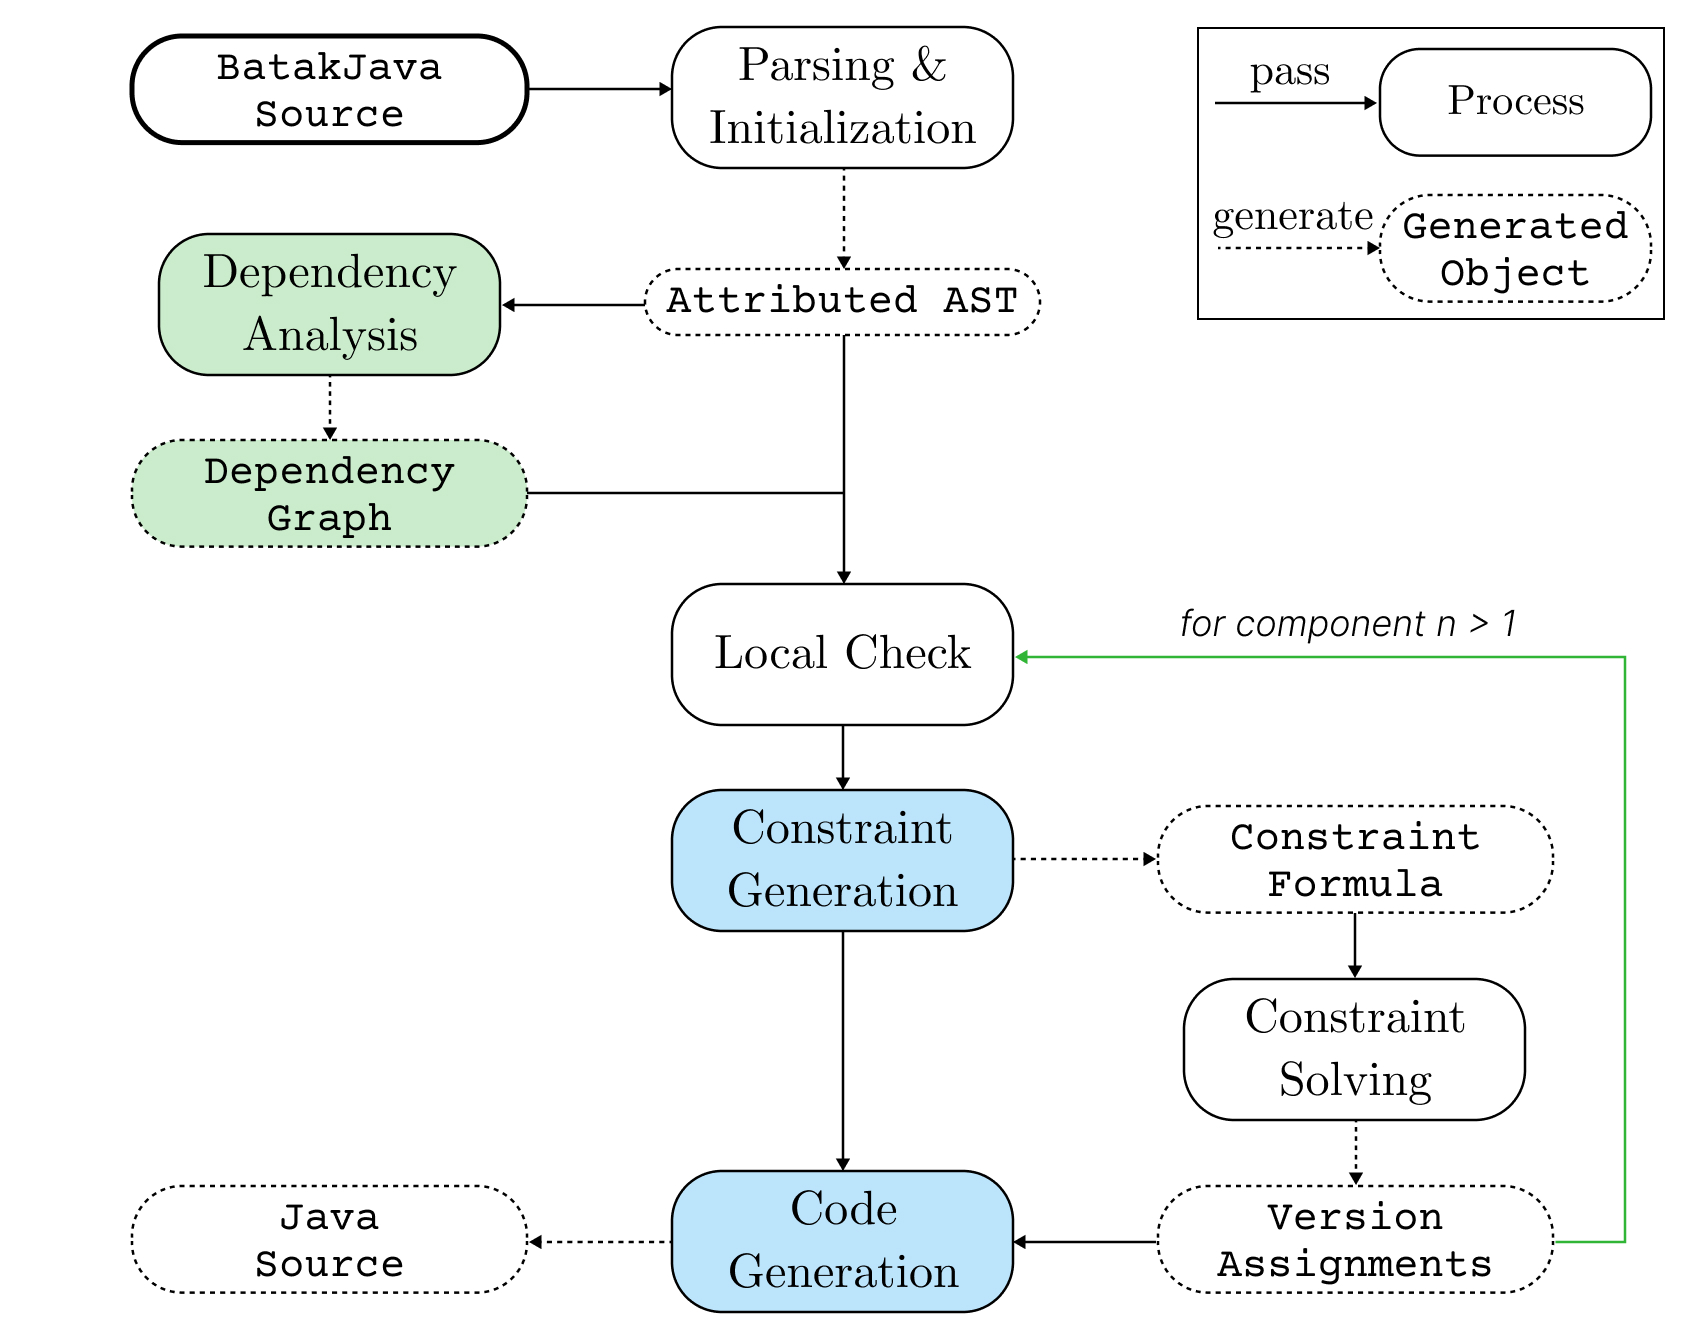
\includegraphics[width=.9\textwidth]{Figures/poly-batakjava.jpg}
\caption{Structure of polymorphic BatakJava's compiler}
\label{poly-bj-overview}
\end{figure}

Polymorphic \lang{} is implemented as an extension of the base \lang{}. 
It is similarly compiled back into Java. 
Figure~\ref{poly-bj-overview} shows the compilation process for a polymorphic BatakJava program. 
There are four main points of modification over the base implementation:
\begin{enumerate}
\item Dependency analysis before local type check
\item Version arguments check on polymorphic instances based on prior solutions
\item Less restrictive component-wise constraint generation
\item Version arguments preserving code generation
\end{enumerate}

\subsection{Dependency Analysis}

Dependency analysis computes the dependency graph that includes the order in which type checking and constraint generation 
of the classes in the program are conducted. The purpose of determining the order is to allow version checking on version 
arguments assigned to class instances.

The dependency relationship is computed using Tarjan’s algorithm~\cite{tarjan1972depth}. 
The algorithm takes the program as input. 
Each (version of) the class declaration \texttt{C ver n} is considered a vertex in the graph. 
Any reference to a class \texttt{D} through class access in a class declaration \texttt{C ver n} 
is considered an edge from the vertex representing \texttt{C ver n} to the vertex representing 
every version of \texttt{D}.
The algorithm outputs the strongly connected components in the graph.
This is described by a list of components consisting of vertices (versioned class declarations) 
and the order of the list. 
Class declarations belonging to the same component contain cyclical references.
The class declarations composing the first component can be considered as the top-most 
module in a dependency relationship. 
Type checking, constraint generation and solving are 
then conducted from the first component.

Figure~\ref{component-hashing} shows the dependency analysis result for the hashing example. 
The arrows show the dependency relation and the dashed lines form the components. 
The program is composed of five components: the first component consists of \texttt{HashValue} 
ver.1 and 2; the second is \texttt{Hash} ver.1; the third is \texttt{Hash} ver.2; the fourth is \texttt{Dir} ver.1; 
the last is \texttt{App}.

\begin{figure}[t]
\center
%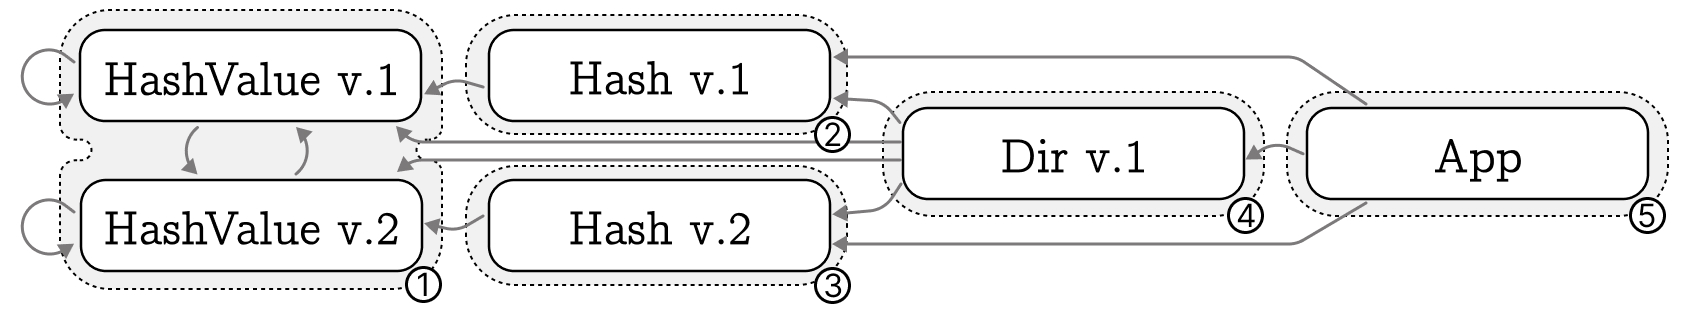
\includegraphics[width=.95\textwidth]{Figures/dependency-component.jpg}
\caption{Dependency analysis result for the hashing example}
\label{component-hashing}
\end{figure}

\subsection{Type Checking}

Polymorphic \lang{} checks the correctness of polymorphic object instantiations. 
This is possible because the dependent classes are already checked and their solutions have been enumerated.
In the hashing example, the polymorphic instance checks are executed in the class \texttt{App}. 
Class \texttt{App} is contained in the last component of the program, therefore during its check the solution 
for class \texttt{Dir} is already available. As mentioned above, the set of solutions $(\texttt{V},\texttt{W})$ was $((1,1),(2,2))$.
Using this set, version arguments on instantiations and invocations are checked. 
Failed checks are considered as type errors.

\subsection{Constraint Generation}

The problem to solve with the constraint generation in the base \lang{} is that 
constraints on type variables are generated globally.
By doing this, the behavior of a class declaration is determined not only by the implementer but
is also affected by how the users instantiate said class declaration.
In the hashing example, the behavior of \texttt{exists} is not determined by the \texttt{Dir} itself, 
but also by how \texttt{new Dir()} in \texttt{App} invokes the method \texttt{exists} (Listing~\ref{app-class}).

Suppose that $e_{1}$ and $e_{2}$ are respectively the body of \texttt{processID} and \texttt{processLog} in 
Listing~\ref{app-class}, these expressions will generate the following constraints in \lang{}, where 
\texttt{T}$_{\texttt{HashValue}}$ is the type variable assigned to the parameter \texttt{c} of the method \texttt{exists}.
\begin{align*}
e_{1} : \texttt{T}_{e_{1}} \mid \: \mathcal{R}_{1} \otimes \{ \texttt{T}_{\texttt{HashValue}} = \texttt{HashValue!1} \} \\
e_{2} : \texttt{T}_{e_{2}} \mid \: \mathcal{R}_{2} \otimes \{ \texttt{T}_{\texttt{HashValue}} = \texttt{HashValue!2} \}
\end{align*}

Eventually, the constraint for the whole program would have the following unsolvable constraint as its subconstraint
\begin{align*}
\mathcal{R}_{1} \otimes \mathcal{R}_{2} \otimes \{ \texttt{T}_{\texttt{HashValue}} = \texttt{HashValue!1} 
\wedge \texttt{T}_{\texttt{HashValue}} = \texttt{HashValue!2} \}
\end{align*}

Polymorphic \lang{} solves this by generating constraints and solving them component-wise. 
The order of components follows the result of the dependency analysis.

In the hashing example, constraints on \texttt{Dir} are already solved by the point \texttt{Dir} instances in 
\texttt{App} are checked. The expressions $e_{1}$ and $e_{2}$ therefore do not add constraints to the definition 
of class \texttt{Dir}. 
Concretely the new constraint generated by $e_{1}$ and $e_{2}$ do not constrain the parameter \texttt{exists}
\begin{align*}
e_{1} : \texttt{T}_{e_{1}} \mid \: \mathcal{R}_{1} \\
e_{2} : \texttt{T}_{e_{2}} \mid \: \mathcal{R}_{2}
\end{align*}

The conjunction of the new sub-constraints which have to be solved is the following constraint.
\begin{align*}
\mathcal{R}_{1} \otimes \mathcal{R}_{2}
\end{align*}

\subsection{Code Generation}

The key change in polymorphic \lang{}'s code generation is by relaxing the code fixing on class access in the 
resulting Java code. 

Specifically in the base \lang{}, Java code is generated naively. The code generation selects one version assignment 
and transpiles the code into Java by fixing class access with the selected version assignments. 
Simply applying the new constraint generation approach described above to collect all the versions assignments 
is not enough to solve the issue because every class access in the code would still be fixed to one version.
For example, the resulting Java code for \texttt{Dir} shown in 
Listing~\ref{pbj-example-code-generation} will still not compile into bytecode due to type incompatibility. 
Specifically in this example, the \texttt{Hash} and \texttt{HashValue} in the method \texttt{exists} is fixed to version 1.
\begin{lstlisting}[
  language=Java,
  caption=A section of code generation result for the hashing example,
  label=pbj-example-code-generation,
  frame=lines
]
class Dir_v1 {
  ...
  boolean exists(HashValue_v1 c) {
    Hash_v1 hash = new Hash_v1();
    ...
  }
}
\end{lstlisting}

In the following section we will demonstrate the transpilation in polymorphic \lang{} by syntactic constructs.

\subsubsection*{Transpiling Class Declarations and Instantiations}

The code generation for class declarations defines an interface for each set of versioned classes. In the 
example, an interface for every class \texttt{Hash}, \texttt{HashValue}, \texttt{Dir}, and \texttt{App} are 
added during code generation. 
The interface plays the role of version polymorphic classes after transpilation.
Each specific version of the class is renamed similarly as in base \lang{}, 
for example \texttt{Hash} version 1 is renamed into \texttt{Hash\_v1} in Java 
and also made to implement the newly added interfaces. 
By doing so, it is possible to pass any specific version of a class as an argument to a version polymorphic parameter.
Listing~\ref{interface-code-generation} shows the headers for \texttt{Hash} and \texttt{Dir}.

Versions for class access in the program, excluding class instantiations and cast expressions are not fixed 
during transpilation as shown in Listing~\ref{dir-renamed-code-generation}.

\begin{figure}[h!]
\begin{lstlisting}[
  language=Java,
  caption=Partial transpilation of \texttt{exists},
  label=dir-renamed-code-generation]
boolean exists(HashValue c) {
  Hash hash = ...;
  ...
}
\end{lstlisting}

\begin{lstlisting}[
  language=Java,
  caption=Header for \texttt{Hash} and \texttt{Dir},
  label=interface-code-generation
]
interface Hash {...}

class Hash_v1 implements Hash {...}

class Hash_v2 implements Hash {...}

interface Dir {...}

class Dir_v1 implements Dir {...}
\end{lstlisting}

\begin{lstlisting}[
  language=Java,
  caption=Transpilation of version parameters in \texttt{Dir},
  label=dir-version-param-code-generation
]
class Dir_v1 {
  Hash_Factory V;
  HashValue_Factory W;
  Dir_v1(Hash_Factory V, HashValue_Factory W) {
    this.V = V; this.W = W;
  }
  boolean exists(HashValue c) {
    Hash hash = ...;
    for (String s: getFiles()) {
      if (hash.match(s, c)) { return true; }
    }
    return false;
  }
}
\end{lstlisting}

\begin{lstlisting}[
    language=Java,
    caption=Factory classes for \texttt{Hash},
    label=factory-class-code-generation
]
interface Hash_Factory {
  Hash make();
}

class Hash_v1_Factory implements Hash_Factory {
  Hash make() { return new Hash_v1(); }
}

class Hash_v2_Factory implements Hash_Factory {
  Hash make() { return new Hash_v2(); }
}
\end{lstlisting}
\end{figure}

In method \texttt{exists}, the versions for the polymorphic \texttt{Hash} and \texttt{HashValue} are not fixed 
allowing us during runtime to pass any version of \texttt{HashValue} as an argument for invoking \texttt{exists}. 
Version checking has been done during the previous step, so erasing version information 
(the parameter \texttt{V} in \texttt{HashValue\#V\#}) 
from the signature during this step will not cause a problem.

Version parameters and arguments are converted into Java objects with \emph{factory interfaces} and 
\emph{factory classes}. In class \texttt{Dir}, versin parameters \texttt{V} and \texttt{W} are respectively converted into 
factory interfaces for \texttt{Hash} and \texttt{HashValue}. Listing~\ref{dir-version-param-code-generation} 
shows the converted parameters \texttt{V} and \texttt{W} as new fields with type \texttt{Hash\_Factory} and 
\texttt{HashValue\_} \texttt{Factory} in \texttt{Dir\_v1}. 
The constructor defined in \texttt{Dir} is correspondingly modified to initialize the new fields for version parameters.

Listing~\ref{factory-class-code-generation} shows the definition of the factory interfaces and factory classes 
with specific versions for \texttt{Hash}. The interface \texttt{Hash\_Factory} defines a method \texttt{make} 
that returns a \texttt{Hash} object. Each specific version of the factory \texttt{Hash\_v1\_Factory} and 
\texttt{Hash\_v2\_Factory} implements the method \texttt{make} by constructing the object in its specific version.

Object instantiations such as \texttt{new Hash\#V\#()} whose version is determined dynamically 
can preserve its version argument information in Java through the use of factory classes. 
In \texttt{Dir\_v1} in Listing~\ref{make-code-generation}, the object instantiation \texttt{new Hash\#V\#()} is 
converted into a \texttt{make} call on the factory object \texttt{V}. 
Specific version arguments such as \texttt{<<1,1>>} in the class \texttt{App} are converted into 
constructor arguments with specific factory classes namely \texttt{new Hash\_v2\_Factory()} and 
\texttt{new Hash\_v1\_Factory()}.

\begin{figure}[t]
\begin{lstlisting}[
  language=Java,
  caption=Runtime object instantiation,
  label=make-code-generation
]
class Dir_v1 {
  ...
  boolean exists(HashValue c) {
    Hash hash = V.make();
  }
}

class App_v1 {
  boolean processID(String n) {
    return new Dir_v1(new Hash_v1_Factory(),
                      new Hash_v1_Factory())
      .mkHash(s);
  }
  boolean processLog(String n) {
    return new Dir_v1(new Hash_v2_Factory(), 
                      new Hash_v2_Factory())
      .mkHash(s);
  }
}
\end{lstlisting}
\end{figure}

\subsubsection*{Transpiling Method Declarations and Invocations}

Code generation for methods require modifications in regards to handling the generated interfaces. 
We illustrate this with the example in Listing~\ref{hash-new-method}, where we add a new version 
of \texttt{Hash} with a new method \texttt{matchWith} while maintaining older methods.

Listing~\ref{hash-new-use} shows a situation where a new version of \texttt{Hash} may be used 
together with an older version of \texttt{Hash}. 
Two polymorphic instances of \texttt{Hash} are defined where different methods are invoked on 
each instance. 

\begin{figure}[t]
\begin{lstlisting}[
    language=Java,
    caption=A new \texttt{Hash} with a different method,
    label=hash-new-method]
class Hash ver 3 {
  ...
  HashValue#2# mkHash(String s) {...}
  boolean match(String s, HashValue#2# h) { ... }
  boolean matchWith(String s, HashValue#2# h) { ... }
}
\end{lstlisting}

\begin{lstlisting}[
    language=Java,
    caption=Using the new \texttt{Hash},
    label=hash-new-use]
# In BatakJava
Hash#V# h1 = new Hash#V#(...);
Hash#W# h2 = new Hash#W#(...);
h1.match("some string", h2.mkHash("some string"));
h2.matchWith("some string", h1.mkHash("some string"));
\end{lstlisting}

\begin{lstlisting}[
    language=Java,
    caption=Transpilation of the code using the new \texttt{Hash},
    label=hash-new-use-transpiled]
# In Java
Hash h1 = V.make(...);
Hash h2 = W.make(...);
h1.match("some string", h2.mkHash("some string"));
h2.matchWith("some string", h1.mkHash("some string"));
\end{lstlisting}
\end{figure}

Suppose that Listing~\ref{hash-new-use} checks and a solution is available for \texttt{V} and \texttt{W}, 
then the resulting transpilation is the code shown in Listing~\ref{hash-new-use-transpiled}.
Here we can observe that the polymorphic class \texttt{Hash\#V\#} and \texttt{Hash\#W\#} 
on variables \texttt{h1} and \texttt{h2} are converted into interface types \texttt{Hash}. 
Following that, methods are invoked against these interface types. 
To allow the resulting code to compile and run in Java, all method declarations in each specific version 
need to be gathered in the interface and implementations for these methods are added 
retrospectively in all the specific versions that do not implement the methods.

Listing~\ref{new-hash-transpiled} shows how methods for \texttt{Hash} are all aggregated in the interface. 
The method \texttt{matchWith} missing in the older versions of \texttt{Hash} are correspondingly 
added the older versions with a default implementation that can be ignored. 
Again, since version checks have been conducted in the previous step, there should not be any 
invocation of \texttt{matchWith} from any \texttt{Hash} objects from ver.1 and 2.

Suppose that the additional method shared the same name and parameters, but with different 
return type as shown in Listing~\ref{hash-new-return}. 
\begin{lstlisting}[
  language=Java,
  caption=A new \texttt{Hash} with overlapping name and a different return type,
  label=hash-new-return,
  frame=lines]
class Hash ver 3 {
  MyBoolean match(String s, HashValue h) { ... }
}
\end{lstlisting}
The transpilation will rename the method into \texttt{match\_\_MyBoolean} and if necessary 
replace any method invocations with the new method name.

\begin{figure}[h!]
\begin{lstlisting}[
    language=Java,
    caption=Transpiling \texttt{Hash}es with different methods,
    label=new-hash-transpiled,
    frame=lines]
interface Hash {
  // from Hash ver.1-3
  HashValue mkHash(String s);
  // from Hash ver.1-3
  boolean match(String s, HashValue h);
  // from Hash ver.3
  boolean matchWith(String s, HashValue h);
}

class Hash_v1 {
  Hash_v1() { }
  HashValue mkHash(String s) { ... }
  boolean match(String s, HashValue h) { ... }
  boolean matchWith(String s, HashValue h) {
    return false;
  }
}

class Hash_v2 {
  Hash_v2() { }
  HashValue mkHash(String s) { ... }
  boolean match(String s, HashValue h) { ... }
  boolean matchWith(String s, HashValue h) {
    return false;
  }
}

class Hash_v3 {
  Hash_v3() { }
  HashValue mkHash(String s) { ... }
  boolean match(String s, HashValue h) {
    return false;
  }
  boolean matchWith(String s, HashValue h) { ... }
}
\end{lstlisting}
\end{figure}

\subsubsection*{Transpiling Field Declarations and Access}

Similar concerns arise with accessing fields on version polymorphic instances. 
As class access are converted into Java's interface types, 
field access in \lang{} need to converted into method calls in Java.

We illustrate this through the field \texttt{val} in class \texttt{HashValue}. 
Listing~\ref{hash-field} shows the definition for two versions of \texttt{HashValue} 
with one containing the instance variable \texttt{val} 
and their use in the \texttt{main} method.

The resulting transpilation is shown in Listing~\ref{hash-field-transpiled}. 
Getter (\texttt{get\_\_<field\_name>}) and setter (\texttt{set\_\_<field\_name>}) 
methods are generated according to instance variables declared in the class. 
With the addition of methods in the transpilation of the specific class, 
those additional methods are also added to the interface and other version 
of the class where the fields are not defined. 

\begin{figure}[h!]
\begin{lstlisting}[
    language=Java,
    caption=Field access and assignment on a \texttt{HashValue} object,
    label=hash-field,
    frame=topline]
class HashValue ver 1 { }

class HashValue ver 2 {
  int val;
}

void main(String[] args) {
  HashValue#V# h = new HashValue#V#(10);
  int hv = h.val;
  h.val = 20;
}
\end{lstlisting}

\begin{lstlisting}[
    language=Java,
    caption=Transpilation of field access and assignment on \texttt{HashValue},
    label=hash-field-transpiled,
    frame=bottomline]
interface HashValue {
  int get__val();
  int set__val(int toAssign);
}

class HashValue_v1 implements HashValue {
  int get__val() { return 0; }
  int set__val(int toAssign) { return 0; }
}

class HashValue_v2 implements HashValue {
  int val;
  int get__val() { return this.val; }
  int set__val(int toAssign) { return this.val = toAssign; }
}

void main(String[] args) {
  HashValue h = V.make(10);
  int hv = h.get__val();
  set__val(20);
}
\end{lstlisting}
\end{figure}

Same-named fields in newer versions with different types or fields shadowing 
other fields in the parent class are handled the same way as the methods 
with different return types, by properly renaming and replacing field access 
with the renamed method calls.